\documentclass[addpoints,10pt]{exam}

\usepackage{amsmath,amsthm,amssymb,amsfonts,mathtools}
\usepackage{enumitem,wrapfig,graphicx}
\usepackage[mathscr]{euscript}
\usepackage{xparse}
\usepackage{cancel}
\usepackage{geometry}
\usepackage[T1]{fontenc}
\renewcommand{\rmdefault}{ptm}
\usepackage{bm}
\usepackage{sectsty}
\usepackage{pgfplots}
\pgfplotsset{compat=1.18}
\usetikzlibrary{arrows.meta}
\usepackage{xcolor}
\definecolor{darkpastelgreen}{rgb}{0.01,0.75,0.24}
\definecolor{blue-violet}{rgb}{0.54,0.17,0.89}
\usepackage{polynom}
\usepackage{parskip}
\usepackage{setspace}

\newcounter{cprob}
\newenvironment{cprob}[1]{%
    \setcounter{cprob}{#1}%
    \noindent\textbf{Problem \thecprob.}%
}{%
    \par\bigskip
}

\theoremstyle{plain}
\newcommand{\theoremname}{Theorem}
\newtheorem{thm}{\protect\theoremname}
\theoremstyle{definition}
\newtheorem{prob}[thm]{Problem}
\newtheorem*{problem*}{Open Problem}
\theoremstyle{plain}
\newtheorem{conjecture}[thm]{Conjecture}
\newtheorem{lem}[thm]{Lemma}
\newtheorem*{lem*}{Lemma}
\newtheorem{obs}[thm]{Observation}
\newtheorem{cor}[thm]{Corollary}
\theoremstyle{definition}
\newtheorem{definition}[thm]{Definition}
\newtheorem{construction}{Construction}

\let\oldprob\prob
\let\endoldprob\endprob
\renewenvironment{prob}
  {\begin{singlespace}\oldprob}
  {\endoldprob\end{singlespace}}

\newcommand{\belowtitle}{\leavevmode\newline}
\newcommand{\Observe}{\text{Observe.}}
\newcommand{\IF}{\mathbf{(\Rightarrow)}}
\newcommand{\FI}{\mathbf{(\Leftarrow)}}
\newcommand{\class}[2][]{\ensuremath{\left[\,#2\,\right]_{#1}}}
\newcommand{\horrule}[1]{\rule{\linewidth}{#1}}
\newcommand{\kkk}{\ensuremath{\Bbbk}}
\newcommand{\CC}{\ensuremath{\mathbb{C}}}
\newcommand{\FF}{\ensuremath{\mathbb{F}}}
\newcommand{\KK}{\ensuremath{\mathbb{K}}}
\newcommand{\NN}{\ensuremath{\mathbb{N}}}
\newcommand{\QQ}{\ensuremath{\mathbb{Q}}}
\newcommand{\RR}{\ensuremath{\mathbb{R}}}
\newcommand{\ZZ}{\ensuremath{\mathbb{Z}}}
\newcommand{\MM}{\ensuremath{\mathcal{M}}}
\newcommand{\TT}{\ensuremath{\mathcal{T}}}
\newcommand{\BB}{\ensuremath{\mathcal{B}}}
\newcommand{\VV}{\ensuremath{\mathcal{V}}}
\newcommand{\WW}{\ensuremath{\mathcal{W}}}
\newcommand{\UU}{\ensuremath{\mathcal{U}}}
\newcommand{\PP}{\ensuremath{\mathcal{P}}}
\newcommand{\LL}{\ensuremath{\mathcal{L}}}
\newcommand{\kk}{\ensuremath{\mathbb{k}}}
\newcommand{\EE}{\ensuremath{\mathbb{E}}}
\newcommand{\Ss}{\ensuremath{\mathcal{S}}}
\DeclarePairedDelimiter{\ip}{\langle}{\rangle}
\DeclarePairedDelimiter{\norm}{\lVert}{\rVert}
\DeclarePairedDelimiter{\sqb}{\lbrack}{\rbrack}
\newcommand{\floor}[1]{\left\lfloor #1\right\rfloor}
\newcommand{\ceil}[1]{\left\lceil #1\right\rceil}
\newcommand{\mbf}[1]{\ensuremath{\mathbf{#1}}}
\newcommand{\tbf}[1]{\textbf{#1}}
\newcommand{\Span}{\ensuremath{\mathrm{Span}}}
\newcommand{\Char}[1]{\mathrm{Char}\,#1}
\DeclareMathOperator{\lcm}{lcm}
\newcommand{\id}{\ensuremath{\mathrm{id}}}
\newcommand{\Gal}[2]{\mathrm{Gal}(#1/#2)}
\newcommand{\Aut}{\ensuremath{\mathrm{Aut}}}
\newcommand{\Fix}[2]{\mathrm{Fix}_{#1}(#2)}
\newcommand{\nil}{\ensuremath{\mathrm{nil}}}
\newcommand{\Hom}{\ensuremath{\mathrm{Hom}}}
\newcommand{\Obj}{\ensuremath{\mathrm{Obj}}}
\newcommand{\Rng}{\ensuremath{\mathrm{Rng}}}
\newcommand{\Ring}{\ensuremath{\mathrm{Ring}}}
\newcommand{\im}{\ensuremath{\mathrm{im}}}
\newcommand{\proj}[2]{\operatorname{proj}_{#1}(#2)}

\newcommand{\StudentName}{Danny Banegas}
\newcommand{\AssignmentName}{Homework 2}
\newcommand{\CourseName}{MATH 746 - Topology I}

\pagestyle{headandfoot}
\runningheadrule
\firstpageheadrule
\firstpageheader{\CourseName}{\StudentName}{\AssignmentName}
\runningheader{\CourseName}{\StudentName}{\AssignmentName}
\firstpagefooter{}{\thepage}{}
\runningfooter{}{\thepage}{}
\printanswers
\DeclareMathAlphabet{\mathcal}{OMS}{cmsy}{m}{n}

\begin{document}

\begin{lem}\label{lem:hausclosedcompact}
  Any closed subset of a compact space is compact. 
\end{lem}
  \begin{proof}
    Consider any open cover $\{U_{\alpha}\}$ of $C$. Since $C$ is closed, $K\setminus{C}$ is open. So then $\{U_{\alpha}\}\cup \{K\setminus C\}$ must be an open cover for all of $K$. Since $K$ is compact, there exists some finite subcover of $\{U_{\alpha}\}\cup \{K\setminus C\}$ which covers all of $K$. Well, $C\subseteq K$, so this finite subcover must cover $C$ as well.
    
    Note that $K\setminus C$ cannot cover $C\subseteq K$ and therefore can't cover all of $K$. So some subset of $\{U_{\alpha}\}$ must be included in this subcover. Let $\{U_{\alpha_{i}}\}_{i=1}^{n}$ be this subset. If $X\setminus C$ is in this subcover, notice that $X\setminus C$ is disjoint from $C$, and so $\{U_{\alpha_{i}}\}_{i=1}^{n}$ must cover $C$. Otherwise we once again have that $\{U_{\alpha_{i}}\}_{i=1}^{n}$ covers $K$ and therefore $C$.
    
    So any open cover $\{U_{\alpha}\}$ of $C$ has a finite subcover, and therefore $C$ is compact.

  \end{proof}


\begin{lem}\label{lem:contimcom}
  The continuous image of a compact set is compact. 
\end{lem}
  \begin{proof}
    Let $K$ be a compact set in $X$ and $f:K\to Y$ a continuous map. Now consider any open cover $\{U_{\alpha}\}$ of $f(K)$. Since $f$ is continuous, each preimage $f^{-1}(U_{\alpha})$ is open in $K$. Now, $\forall x\in K$, $f(x)\in U_{\alpha}$ for some $\alpha$. Therefore, $x\in f^{-1}(U_{\alpha})$, and we see that $\{f^{-1}(U_{\alpha})\}$ is an open cover for $K$. Then since $K$ is compact, there exists a finite subcover $\{f^{-1}(U_{\alpha_{i}})\}_{i=1}^{n}\subseteq \{f^{-1}(U_{\alpha})\}$. 
    
    Finally, $K\subseteq \bigcup_{i=1}^{n} f^{-1}(U_{\alpha_{i}})\implies f(K)\subseteq \bigcup_{i=1}^{n}f(f^{-1}(U_{\alpha_{i}}))= \bigcup_{i=1}^{n}U_{\alpha_{i}}\implies \{U_{\alpha_{i}}\}_{i=1}^{n}\subseteq \{U_{\alpha}\}$ is a finite subcover. So any open cover $\{U_{\alpha}\}$ of $f(K)$ has a finite subcover, and therefore $f(K)$ is compact.

  \end{proof}

\begin{lem}\label{lem:comhausclosed}
  Any compact subset of a Hausdorff space is closed.
\end{lem}
  \begin{proof}
    Let $H$ be Hausdorff and $K\subseteq H$ a compact subset. We show that $H\setminus K$ is open. 

    Since $H$ is Hausdorff, for each $x\in H\setminus K$ and each $k\in K$, we can find disjoint open sets $U_{k}(x),V_{k}$ containing $x$ and $k$, respectively. Now, $\{V_{k}\mid k\in K\}$ is an open cover of $K$, and since $K$ is compact there exists a finite subcover $\{V_{k_{i}}\}_{i=1}^{n}\subseteq {V_{k}}$. Set $U_{x}=\bigcap_{i=1}^{n}U_{k_{i}}(x)$ and recall that $U_{k_{i}}(x)\ni x$ is disjoint with $V_{k_{i}}$ for each $i\in [n]$. 
    
    So by construction, $U_{x}$ is disjoint from $\bigcup_{i=1}^{n} V_{k_{i}}\supseteq K$ placing it completely inside $H\setminus K.$ That is, $U_{x}\subseteq H\setminus K,\;\forall x\in H\setminus K$. On the otherhand, $x\in U_{x},\forall x\in H\setminus K\implies H\setminus K\subseteq \bigcup_{x\in H\setminus K}U_{x}.$

    Finally, we see that then $H\setminus K=\bigcup_{x\in H\setminus K} U_{x}$, an arbitrary union of open sets, which implies that $H\setminus K$. Therefore, it's complement $K$ must be closed.

  \end{proof}

    \begin{thm}\label{thm:contimjhom} If $f:X\hookrightarrow Y$ is a continuous injection where $X$ is compact and $Y$ is Hausdorff, then $X\cong f(X)$. If $f$ is surjective then $f$ is a homeomorphism.
    \end{thm}
  \begin{proof}
    Since $f$ is injective, $X$ is in bijection with its image $f(X)$. So we show $f^{-1}:f(X)\to X$ is continuous by showing the preimage of every closed set is closed.

    Consider any closed subset $C\subseteq X$. Since $X$ is compact, by \textbf{Lemma }\ref{lem:hausclosedcompact} we have that $C$ is also compact. Then, since $f$ is continuous, by \textbf{Lemma }\ref{lem:contimcom}, the continuous image (and preimage of $C$ via $f^{-1}$) $f(C)$ of the compact set $C$ is also compact. Finally, by \textbf{Lemma }\ref{lem:comhausclosed}, any compact subset of a Hausdorff space is closed. So $f(C)\subseteq f(X)\subseteq Y\implies f(C)$ is closed. So we see the preimage $(f^{-1})^{-1}(C)=f(C)$ of any closed set via $f^{-1}$ is closed, and so $f^{-1}$ is also continuous. 
    
    So $f$ is a bicontinuous bijection from $X$ to $f(X)$, or equivalently, $f$ is a homeomorphism from $X$ to its image and $X\cong f(X)$. Finally, if $f(X)=Y$ of course $f$ is a homeomorphism from $X$ to $Y$.

  \end{proof}

\begin{obs}\label{obs:ballinsub}
If $X$ is a subspace of $\RR^{n}$, and $V$ is open in $X$, then for all $x\in U$ there exists $\varepsilon>0$ small enough that $U_{x}=(B_{\varepsilon}(x)\cap X)\subseteq U$ is an open subneighborhood of $x$ in $X$.
\end{obs}
  \begin{proof}
    By definition since $X$ is a subspace, $U$ can be decomposed as $O\cap X$ for some open set $O$ of $\RR^{n}$ and since $x$ is an interior point of $O$ in $\RR^{n}$ there exists $\varepsilon>0$ such that $B_{\varepsilon}(x)\subseteq O$, and so $x\in U_{x}=(B_{x}(x)\cap T)\subseteq (O\cap X)=U.$
  \end{proof}

%%%%%%%%%%%%%%%%%%%%%%%%%%%%%%%%%%%%%%%%%%%% problem 1 %%%%%%%%%%%%%%%%%%%%%%%%%%%%%%
\setcounter{thm}{0}
\begin{prob}
Show that local compactness is invariant under continuous open mappings.
\end{prob}

\begin{proof}
Let $f:X\to Y$ be a continuous open map, and $X$ a locally compact space. Consider any $x\in X$. By definition $x\in U\subseteq K$ where $U$ is open and $K$ is compact. Since $f$ is a continuous open map, we also have that $f(U)$ is open and then also the continuous image of a compact set is compact by \textbf{Lemma }\ref{lem:contimcom}, so $f(K)$ is compact. So in fact the statement is immediate; $f(x)\in f(U)\subseteq f(K)\subseteq Y$ and $f(U)$ is open, $f(K)$ is compact.

\end{proof}
%%%%%%%%%%%%%%%%%%%%%%%%%%%%%%%%%%%%%%%%%%%% problem 2 %%%%%%%%%%%%%%%%%%%%%%%%%%%%%%

\begin{prob}
Let $\{X_{\alpha}\}$ be an indexed family of non-empty sets. Show that
$\prod_{\alpha}X_{\alpha}$ is locally compact if and only if each
$X_{\alpha}$ is locally compact and $X_{\alpha}$ is compact for all but
finitely many values of $\alpha$. (You may assume the Tychonoff Theorem.)
\end{prob}

\begin{proof}
$(\implies)$ Suppose that $X=\prod_{\alpha}X_{\alpha}$ is locally compact. Each
coordinate projection $\pi_{\alpha}\colon X\to X_{\alpha}$ is a continuous open surjection. The preimage of any open set $U_{\alpha}\subseteq X_{\alpha}$ via $\pi_{\alpha}$ must be all of $X$ with points in the $\alpha$-coordinate belonging to $U_{\alpha}$ and then of course any open set of $X$ either has $X_{\alpha}$ or some open set $U_{\alpha}$ in the $\alpha$-coordinate so its image via $\pi_{\alpha}$ is either $U_{\alpha}$ or all of $X_{\alpha}$. It is trivial the map is a surjection. Problem 1 then gives that every $X_{\alpha}$ is locally
compact.

Fix some $x\in X$. $X$ is locally compact so $x\subseteq U\subseteq K$ where $U,K$ are open and compact, respectively. Well, the $\alpha$-coordinate of $U$ is $X_{\alpha}$ for all but finitely many $\alpha$, and so $\pi_{\alpha}(U)=X_{\alpha}$ for all but finitely many $\alpha$. The map is surjective so $\forall y\in X_{\alpha}, \exists x\in X$ such that $y=\pi_{\alpha}(x)\subseteq \pi_{\alpha}(U)=X_{\alpha}\subseteq \pi_{\alpha}(K)$ and we have that $\pi_{\alpha}(K)=X_{\alpha}$, for all but finitely many $\alpha$. As previously established $\pi_{\alpha}(K)$ is compact so $X_{\alpha}$ must be compact for all but finitely many $\alpha$. 

$(\impliedby)$ On the other hand, suppose every $X_{\alpha}$ is locally compact and that for a finite set $F$, $X_{\alpha}$ is compact whenever
$\alpha\notin F$. Fix $x=(x_{\alpha})\in X$. Once again, $\forall \alpha\in F,\forall x\in X_{\alpha}$ we have $x\subseteq U_{\alpha}\subseteq K_{\alpha}$ which are open and compact, respectively. Now set $U_{\alpha}=K_{\alpha}=X_{\alpha},\forall \alpha\notin F.$ All $K_{\alpha}$ are compact, so by the Tychonoff Theorem,
$K=\prod_{\alpha}K_{\alpha}$ is compact. Also $x_{\alpha}\in U_{\alpha}\subseteq K_{\alpha},\;\forall \alpha$. So then $x=(x_{\alpha})\in U=\prod_{\alpha}U_{\alpha}\subseteq K=\prod_{\alpha} K$ and $U$ is open. So we see $X$ is locally compact.

\end{proof}
\newpage
%%%%%%%%%%%%%%%%%%%%%%%%%%%%%%%%%%%%%%%%%%%% problem 3 %%%%%%%%%%%%%%%%%%%%%%%%%%%%%%

\begin{prob}
Let $\{(X_i,\tau_i)\}_{i\in I}$ be a family of topological spaces and define
the box topology on $\prod_{i\in I}X_i$ as the topology generated by the set
\[
\left\{\prod_{i\in I}U_i\,\middle|\,U_i\in\tau_i\right\}.
\]
\begin{enumerate}[label=(\alph*)]
    \item Show that the product of compact topological spaces, endowed with
    the box topology, is not necessarily compact.
    \item Let $X$ be a topological space. We endow
    $X^{\NN}=\prod_{i\in\NN}X$ with the box topology. Is the diagonal map
    \[
    \Delta:X\longrightarrow X^{\NN}\text{defined by }
    x\longmapsto (x,x,x,\ldots)
    \]
    continuous?
\end{enumerate}
Here I set $\NN=\ZZ^{+}.$
\end{prob}

\begin{proof}
    (a) Consider $\left\{X_{i}=\{0,1\}\right\}_{i\in \NN}$ where each copy of $\{0,1\}$ has the discrete topology. Recall that singletons are open in each copy and in fact form a basis. In the box topology on
    $X=\prod_{i\in\NN}X_i$, every singleton is open, since for all $x=(x_{i})_{i\in \NN}\in X,$
    \[
    \{x\}=\prod_{i\in\NN}\{x_i\} \text{, a product of open sets in each coordinate.}
    \]
    So $X$ inherits the discrete topology, and an open cover for the space is $\{\{x\}\mid x\in X\}$. Well, the space is infinite so no finite subset of singletons can cover the whole space. So we have found an open cover $X$ without a finite subcover and so this box product of compact topological spaces is not
    compact.

    (b) Not in general. Consider $\RR$ (with the standard topology) and $\RR^{\NN}$.
    $B=\prod_{n\in \NN}\left(-\frac1n,\frac1n\right)=(-1,1)\cup (-\frac{1}{2},\frac{1}{2})\cup (-\frac{1}{3},\frac{1}{3}) \cdots$ is open in $\RR^{\NN}$. Now consider $\Delta:\RR\to \RR^{\NN}.$ If $\Delta(x)=(x)_{n\in \NN}\in U=\prod_{n\in \NN} U_{n}$, then $x\in U_{n},\forall n\in \NN$ by definition. So in fact $\Delta^{-1}(U)=\bigcap_{n\in \NN}U_{n}$. Therefore,
    \[
    \Delta^{-1}(B)=\bigcap_{n\in \NN}
    \left(-\frac1n,\frac1n\right)=\{0\},
    \]
    which is not open in $\RR$. So $\Delta:\RR\to \RR^{n}$ is not continuous, and we have found a counterexample. That is, the diagonal map is not always continuous.

\end{proof}
\newpage
%%%%%%%%%%%%%%%%%%%%%%%%%%%%%%%%%% Problem 4%%%%%%%%%%%%%%%%%%%%%%%%%%%%%%%%%%%%%%%%%%%
\begin{prob}
Show that the one-point compactification of $\ZZ_{+}$ is homeomorphic to the
subspace
\[
A=\{0\}\cup\left\{\frac1n\,\middle|\,n\in\ZZ_{+}\right\}
\subset\RR.
\]
\end{prob}

\begin{proof} We take denote the one-point compactification
$\ZZ_{+}^{*}=\ZZ_{+}\cup\{\infty\}$. Since $\ZZ_{+}$ is discrete, its compact
subsets are exactly its finite subsets, since its singletons form a basis. So for all distinct $x,y\in \ZZ_{+}$, $\{x\}\cap \{y\}=\emptyset$, $x\in \{x\}\subseteq \{x\}$ and lastly $\{\{n\}\mid n\in \ZZ_{+}\}$ is a cover of $\ZZ_{+}$ without a finite subcover. So $\ZZ_{+}$ is Hausdorff, locally compact, but not globally compact. Now by definition, a subset $U\subseteq \ZZ_{+}^{*}$ is open if
    \begin{align*}
        U&\text{ is open in }\ZZ_{+}\\
        &\text{ or }\\
        U&=\{\infty\}\cup \ZZ_{+}\setminus K
    \end{align*}
For some compact set $K$ in $\ZZ_{+}$ which must also be closed by \textbf{Theorem }\ref{lem:hausclosedcompact} since $\ZZ_{+}$ is Hausdorff. Notice that then every open set containing $\infty$ must be $\{\infty\}\cup (\ZZ_{+}\setminus F)$ for some finite subset $F\subseteq \ZZ_{+}.$
Next, define $f:\ZZ_{+}^{*}\to A$ by
\[
f(\infty)=0,
\qquad
f(n)=\frac1n.
\]
This is obviously a bijection. Next, consider any open set $U$ in $A$. It must be the intersection of $A$ and some arbitrary union of open intervals in $\RR$. If $U$ doesn't contain $0$, then it must simply by definition be some subset of $A$ which will be $U=\{\frac{1}{n}\}_{n\in I\subseteq \ZZ_{+}}$ and then the preimage $f^{-1}(U)=\{n\}_{I}=I$ is an open set in $\ZZ_{+}$ and therefore an open set in $\ZZ_{+}^{*}.$ Otherwise, $0\in U\implies U=\{0\}\cup\{\frac{1}{n}\}_{n\in I}\implies f^{-1}(U)=\{\infty\}\cup I.$

Now, since $U$ is open all of it's points are interior points and so $0\in U\implies \exists\varepsilon>0$ such that $B_{\varepsilon}(0)\cap A\subseteq U.$ Now, pick some $N\in \ZZ_{+}$ such that $0<\frac{1}{N}<\varepsilon$. (which exists by the \textit{Archemedian Property}) For any $n\geq N$, $0< \frac{1}{n}\leq \frac{1}{N}\leq \varepsilon.$ So $n\in I,\forall n\geq N.$ So then any $m\notin I$ must be such that $0<\frac{1}{N}< \frac{1}{m}$. That is, $0<m<N\implies F=\ZZ_{+}\setminus I\subseteq [N-1].$ Then, we have that $F$ is finite and therefore compact in $\ZZ_{+}$ and by definition $f^{-1}(U)=\{\infty\}\cup I=\{\infty\}\cup (\ZZ_{+}\setminus F)$ where $F$ is compact in $\ZZ_{+}.$ So $f^{-1}(U)$ is open and $f$ is continuous.

Now, consider any $\frac{1}{n}\in A\setminus\{0\}$ for $n>1$. The two closest points in $A\setminus\{0\}=\{\frac{1}{n}\}_{\ZZ_{+}}$ to $\frac{1}{n}$ via the metric in $\RR$ are $\frac{1}{n+1}$ and $\frac{1}{n-1}$. Set $0<\varepsilon<\min\{|\frac{1}{n}-\frac{1}{n+1}|,|\frac{1}{n}-\frac{1}{n-1}|\}$ for $n>1$, otherwise, for $n=1,$ set $0<\varepsilon<1/2$. Notice that $B_{\varepsilon}(\frac{1}{n})=(\frac{1}{n}-\varepsilon,\frac{1}{n}+\varepsilon)$ is open in $\RR$ and in fact since it excludes the closest other points to $\frac{1}{n}$ in $A,\;\forall n\in \ZZ_{+}$. So we have that $B_{\varepsilon}(\frac{1}{n})\cap A=\{\frac{1}{n}\}$ is open for all $\frac{1}{n}\in A\setminus\{0\}.$ So non-zero singletons are open in $A.$
 
 Therefore, for any distinct $\frac{1}{m},\frac{1}{n}\in A\setminus\{0\}$: $\{\frac{1}{m}\}\text{ and }\{\frac{1}{n}\}$ are disjoint open sets, and otherwise for distinct $a,b\in A$ without loss of generality $a=0,b=\frac{1}{n}$ and so pick $0<\varepsilon_{m}<\frac{1}{m}$ and we see that $B_{\varepsilon_{m}}(0)\cap A=\{0\}\cup \{\frac{1}{i}\}_{i> m}$ and $\{\frac{1}{m}\}$ are disjoint open sets. So then $A$ is Hausdorff, and we already have that $\ZZ_{+}^{*}$ is compact. Therefore, $f$ is a continuous bijection from a compact space to a Hausdorff space, and so finally by \textbf{Theorem }\ref{thm:contimjhom}, we have that $f$ is a Homeomorphism; $\ZZ_{+}^{*}\cong A=\{0\}\cup \{\frac{1}{n}\}_{\ZZ_{+}}\subseteq \RR.$

\end{proof}
\newpage

\begin{prob}
Let $X$ denote the rational points of the interval
$[0,1]\times\{0\}\subset\RR^2$. Let $T$ denote the union of all line
segments joining the point $p=(0,1)$ to the points of $X$.
\begin{enumerate}[label=(\alph*)]
    \item Show that $T$ is path connected, but it is locally connected only
    at the point $p$.
    \item Find a subset of $\RR^2$ that is path connected but is locally
    connected at none of its points.
\end{enumerate}
\end{prob}

\begin{proof}
(a) Recall the definition of path connectedness: A space $X$ is path connected if $\forall x,y\in X,$ there exists a continuous map $f:[0,1]\to X$ such that $f(0)=x,\;f(1)=y.$  Now consider any $a,b\in T$ and define $f:[0,1]\to T$ as the map that (in this order) sends all points along $[0,1/2]$ to the points along the segment from $a$ to $p$ and then all the points from $[1/2,1]$ to the points along the segment from $p$ to $b$. 

Now, consider any open set in $T$. It is the intersection of some arbitrary union of open balls in $\RR^{2}$ and $T$. The intersection of an open ball and $T$ will just be an arbitrary union of 'subsegments' of $T$ contained in that open ball. 
Well, the only points in $T$ with a preimage via $f$ lie on the segment from $a$ to $p$ or the one from $p$ to $b$. That is, the preimage of any subsegment of a segment other than $[a\to p]$ or $[a\to p]$ is simply $\emptyset$. So pulling back from any open set $U$ of $T$ via $f$, will give us the union of preimages of it's subsegment members, which we just established will only give us the union of preimages of subsegments of $[a\to p]$ and $[p\to b]$ contained in $U.$ Well, the preimages of these are open intervals in $[0,1]$, half open intervals in $[0,1]$, or the whole space, which are all open in $[0,1]$. (We can't form a closed paths using arbitrary unions of open sets in $\RR^{2}$, otherwise we could do so in $\RR$) If no portion of either segment exists in our open set $U$ then its preimage is $\emptyset$ which is open. So $f$ is open for any $x,y\in T$ and $T$ is path connected.

Consider any open neighborhood $U$ of $p$ in $T$, by \textbf{Observation }\ref{obs:ballinsub} we have some $\varepsilon>0$ such that $U_{p}=(B_{\varepsilon}(p)\cap T)\subseteq U$ is an open subneighborhood of $p.$ Well, we just use the same map and argument as before for any distinct $a,b\in U_{\varepsilon}\subseteq U$ (since it always contains $p$) to see that $U_{\varepsilon}\subseteq U$ is a path connected, and therefore connected open subneighborhood of $p$ contained in $U$ satisfying local connectness at $p$ in $T$; We can always draw a path from any point back to $p$ and out to any other point in the same manner as before.

Suppose $T$ is locally connected at any $x\in T\setminus\{p\},$ and choose $\varepsilon>0$ small enough that $p\not\in B_{\varepsilon}(x)$ in $\RR^{2}.$ Then, intersecting with $T$ gives us an open neighborhood $U=B_{\varepsilon}(x)\cap T$ of $x$ in $T$. Now, since $T$ is locally connected at $x$ there exists a connected open subneighborhood $V\subseteq U$ of $x.$ Then by \textbf{Observation }\ref{obs:ballinsub} there exists $\delta>0$ small enough that $V_{x}=B_{\delta}(x)\cap Y\subseteq V$. Now we turn our attention to $B_{\delta}(x)$ in $\RR^{2}.$ By the \textit{Archemedian Property} we have some $M\in \ZZ_{+}$ so that $0<1/M<\delta$ and so a subsegment of the spokes from $p$ to $(\frac{1}{M},0)$ and from $p$ to $(\frac{1}{M+1},0)$ belong to it when intersected with $T$ by definition. Therefore, choose some irrational $\frac{1}{M+1}<c<\frac{1}{M}$ whose spoke doesn't belong to $T.$ The open half planes $H_{L}(c)$ and $H_{R}(c)$ on either side of the line $\ell_{c}$ this spoke belongs to are open in $\RR^{2}$ cover $\RR^{2}$ with the $\ell_{c}$ removed. So then since no point on $\ell_{c}$ is in $V$ by definition since $c$ is irrational, when intersected with $T$ and $V$ they must cover $V$ as well. So we get a decomposition of $V$ into two disjoint open neighborhoods; $V=((H_{L}(c)\cap T)\cap V)\cup ((H_{R}(c)\cap T)\cap V)$, which contradicts that $V$ is connected. So we see $T$ is locally connected at $p$ and nowhere else.

\begin{figure}[h]
    \centering
    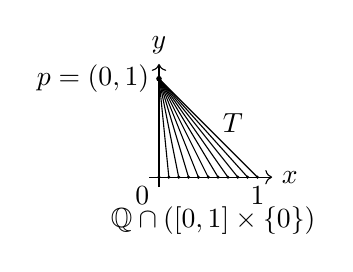
\begin{tikzpicture}[scale=1.25]

        % Axes
        \draw[->] (-0.1,0) -- (1.15,0) node[right] {$x$};
        \draw[->] (0,-0.1) -- (0,1.15) node[above] {$y$};

        % Hub
        \fill (0,1) circle (0.8pt);
        \node[left] at (0,1) {$p=(0,1)$};

        % Representative rational spokes
        \foreach \x in {0,0.1,0.2,0.3,0.4,0.5,0.6,0.7,0.8,0.9,1}
        {
            \draw (0,1) -- (\x,0);
            \fill (\x,0) circle (0.5pt);
        }

        % Labels
        \node[below left] at (0,0) {$0$};
        \node[below] at (1,0) {$1$};
        \node[below] at (0.55,-0.2)
            {$\mathbb{Q}\cap([0,1]\times \{0\})$};

        \node[right] at (0.55,0.55) {$T$};

    \end{tikzpicture}
    \caption{The space $T$, consisting of the line segments from
    $p=(0,1)$ to $(q,0)$ for $q\in\mathbb{Q}\cap[0,1]$.}
\end{figure}

\newpage
(b) Now let $T_{1}=T$ with hub $p_{1}=(0,1)$ and $T_{2}$ be the set of all segments from the hub $p_{2}=(0,0)$ to rational points along $X'=([-1,0]\times \{1\})\subseteq \RR^{2}$. Slide $T_{2}$ up $1$ and reflect about $y=1, x=0$, in that order, to see that $T_{2}\cong T_{1}=T.$ Now consider $Y=T_{1}\cup T_{2}$, a union of two copies $T_{1},T_{2}$ of $T$ joined at their hubs $p_{1},p_{2}$ by a 'spine' subsegment of the $y$-axis. In fact, to be clear: the spine segment $\{0\}\times [0,1]$, which includes both hubs, belongs to both $T_{1}$ and $T_{2}$ already. It is obvious that this space is path connected. Each copy of $T$ was already proven to be path connected, and then we can travel from $x_{1}\in T_{1}$ and $x_{2}\in T_{2}$ or vice versa by traveling from the $x_{1}$-spoke back to $p_{1}$, then traveling from $p_{1}$ to $p_{2}$ along the spine, and then finally we travel from $p_{2}$ out to $x_{2}$; $f([0\to 1/3])=[x_{1}\to p_{1}],f([1/3\to2/3])=([p_{1}\to p_{2}]),f([2/3\to 1])=([p_{2}\to x_{2}])$ is a continuous map by the by a similar argument as those appearing in $(a).$

Now suppose $Y$ is locally connected at any non-hub point $y\in Y\setminus\{p_{1},p_{2}\},$ and choose $\varepsilon>0$ small enough that $B_{\varepsilon}(y)$ contains neither $p_{1}$ nor $p_{2}.$ $U=B_{\varepsilon}(y)\cap Y$ is an open neighborhood of $y$, and by local connectness at $y$ it contains a connected open subneighborhood $V\subseteq U$ of $y$. Next, either $V$ is completely contained in one copy of $T$ or it isn't. If it is, by $(a)$ we get a decomposition of $V$ into two disjoint open sets formed by half planes, contradicting connectedness. Then in fact if $V$ isn't contained in just one copy of $T$ we can make essentially the same argument. Since $V$ is open, we can choose $\delta>0$ small enough that $B_{\delta}(y)\cap Y\subseteq V.$

\begin{figure}[h]
    \centering
    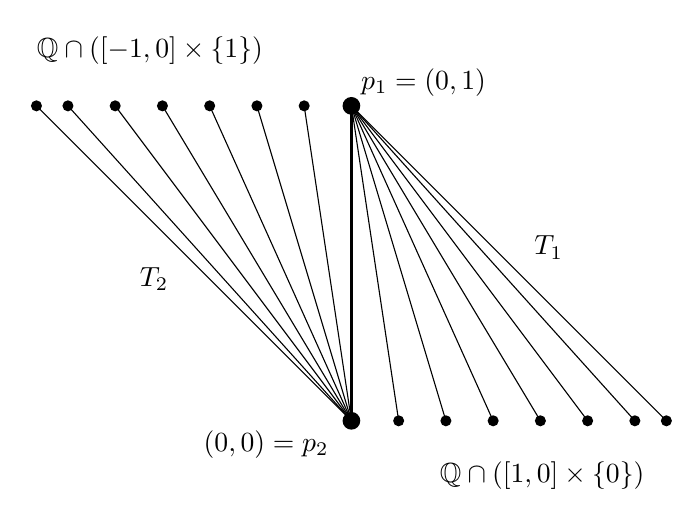
\begin{tikzpicture}[scale=4]

        % Spine
        \draw[very thick] (0,0) -- (0,1);

        % T_1: hub (0,1), endpoints to the right at y=0
        \foreach \x in {0.15,0.3,0.45,0.6,0.75,0.9,1}
        {
            \draw (0,1) -- (\x,0);
            \fill (\x,0) circle (0.5pt);
        }

        % T_2: hub (0,0), endpoints to the left at y=1
        \foreach \x in {-0.15,-0.3,-0.45,-0.6,-0.75,-0.9,-1}
        {
            \draw (0,0) -- (\x,1);
            \fill (\x,1) circle (0.5pt);
        }

        % Hubs
        \fill (0,1) circle (0.8pt);
        \fill (0,0) circle (0.8pt);

        \node[above left] at (-0.25,1.1) {$\QQ\cap ([-1,0]\times \{1\})$};
        \node[above right] at (0,1) {$p_1=(0,1)$};
        \node[below right] at (-0.5,0) {$(0,0)=p_{2}$};
        \node[below right] at (0.25,-0.1) {$\QQ\cap ([1,0]\times \{0\})$};

        % Labels
        \node[right] at (0.55,0.55) {$T_1$};
        \node[left] at (-0.55,0.45) {$T_2$};

    \end{tikzpicture}
    \caption{The space
    $Y=T_1\cup T_2\cup(\{0\}\times[0,1])$.}
\end{figure}
\end{proof}

\begin{prob}
Define the cone $CX$ to be the quotient space obtained by identifying
$X\times\{1\}$ in $X\times[0,1]$ to a point. Prove that $CX$ is path
connected. Deduce that any $X$ is a subspace of a path connected space.
\end{prob}

\begin{proof}
Let $q\colon X\times[0,1]\to CX$ be the quotient map, and let
$v=q(X\times\{1\})$ be the cone point. For any $q(x,t)\in CX$, the map
\[
\gamma_{x,t}(s)=q\bigl(x,(1-s)t+s\bigr),
\qquad 0\leq s\leq1,
\]
is a path from $q(x,t)$ to $v$. Any two points can therefore be joined by
following one such path to $v$ and then following the reverse of another.
Thus $CX$ is path connected.

The set $X\times[0,1)$ is open and saturated for the quotient map, and no two
of its points are identified. Hence the restriction
\[
q\big|_{X\times[0,1)}\colon X\times[0,1)
\longrightarrow CX\setminus\{v\}
\]
is a homeomorphism. In particular, $x\mapsto q(x,0)$ embeds $X$ as the
subspace $q(X\times\{0\})$ of the path connected space $CX$.
\end{proof}

\end{document}
